\section{Setup with WSL}

Follow these steps to set up a Zephyr development environment in the WSL.

\begin{itemize}
  \item Install the \emph{J-Link Software and Documentation pack}.
    Make sure to tick the \emph{Install legacy USB Driver for J-Link (requires admin rights)} checkbox during installation.

    \href{https://www.segger.com/downloads/jlink/JLink_Windows_x86_64.exe}{Download}

  \item Install \emph{PuTTY} or another application that can be used for serial
    communication.
    Either download from \href{https://putty.org/}{here} or install with \emph{winget}:

        \begin{monobox}
winget install --id PuTTY.PuTTY -e
\end{monobox}

  \item Install \href{https://aka.ms/terminal}{\emph{Windows Terminal}} for a better terminal experience.

        \begin{monobox}
winget install --id Microsoft.WindowsTerminal -e
\end{monobox}

  \item Open a terminal.

  \item Ensure that the WSL is installed.
        \begin{monobox}
wsl --install --no-distribution
\end{monobox}

    \begin{infobox}
      After installing WSL, make sure to reboot your machine.
      Otherwise the changes will not be applied.
    \end{infobox}

    \begin{infobox}
      If you see the help output of \mono{wsl} try without the \mono{--no-distribution} switch.
      If you get an error try installing the WSL from the Windows Store.
      This can either be done with the \emph{Microsoft Store} GUI or with \mono{winget}:

          \begin{monobox}
winget install "Windows Subsystem for Linux"
\end{monobox}

    \end{infobox}

  \item Create a folder for the environment and import the provided WSL image.
        \begin{monobox}
mkdir \path\to\wslDistroStorage\@\imagename{}@
wsl --import @\imagename{}@ `
  \path\to\wslDistroStorage\@\imagename{}@ `
  "$env:USERPROFILE\Downloads\@\imagename{}@_wsl.tar.zst"
\end{monobox}

  \item Open a shell inside the environment.

        \begin{monobox}
@\cmdinwsl{}@
\end{monobox}

    \begin{infobox}
      In case you get a \emph{CreateProcessParseCommon:789: Failed to translate D:\textbackslash} error the file system might not be available from within WSL.
      Run the following command to list the available file systems.

      % \cmdinwsl{ls /mnt}
          \begin{monobox}
@\cmdinwsl{}@ ls /mnt
\end{monobox}

      You can try mounting the missing file system (\mono{D:\\} in this case) with the following commands.

          \begin{monobox}
@\cmdinwsl{}@ mkdir /mnt/d
@\cmdinwsl{}@ mount -t drvfs D: /mnt/d
\end{monobox}
    \end{infobox}
    \begin{infobox}
      If you are using \emph{Windows Terminal} you can conveniently open a new tab with the environment.
      You might have to restart the terminal for this option to appear.
      \begin{center}
        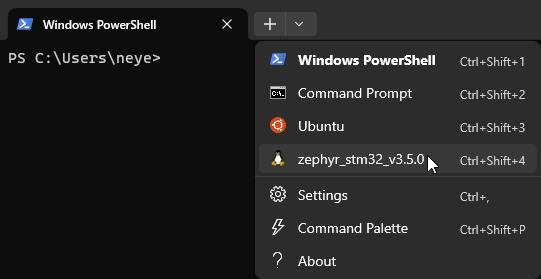
\includegraphics[width=.5\paperwidth]{terminal_open_wsl_tab}
      \end{center}
    \end{infobox}
\end{itemize}
